\documentclass[10pt,twocolumn,letterpaper]{article}

% --- Page Geometry (CVPR/ACL-style two-column conference layout) ---
\usepackage[
  top=0.74in,
  bottom=0.76in,
  left=0.66in,
  right=0.66in,
  columnsep=0.25in
]{geometry}

% --- Float Placement & Spacing Tuning (compact 4-page camera-ready) ---
\renewcommand{\topfraction}{0.92}
\renewcommand{\bottomfraction}{0.85}
\renewcommand{\textfraction}{0.06}
\renewcommand{\floatpagefraction}{0.75}
\renewcommand{\dbltopfraction}{0.92}
\renewcommand{\dblfloatpagefraction}{0.75}
\setcounter{topnumber}{3}
\setcounter{dbltopnumber}{2}
\setlength{\textfloatsep}{7pt plus 2pt minus 2pt}
\setlength{\dbltextfloatsep}{8pt plus 2pt minus 2pt}
\setlength{\floatsep}{6pt plus 2pt minus 2pt}
\setlength{\dblfloatsep}{6pt plus 2pt minus 2pt}

% --- Typography & Micro-typography (BasicTeX 2026 native) ---
\usepackage[T1]{fontenc}
\usepackage[utf8]{inputenc}
\renewcommand{\rmdefault}{ptm}
\usepackage{microtype}

% --- Math ---
\usepackage{amsmath,amssymb,mathtools,bm}

% --- Tables & Colors ---
\usepackage{booktabs}
\usepackage{array}
\usepackage[table,dvipsnames]{xcolor}

% --- Figures & Vector Graphics (TikZ) ---
\usepackage{graphicx}
\usepackage{tikz}
\usetikzlibrary{arrows.meta,positioning,shapes.geometric,fit,backgrounds,calc}
\usepackage[font=small,labelfont=bf,labelsep=period,skip=5pt]{caption}
\usepackage{subcaption}

% --- Hyperlinks & Citations ---
\usepackage[numbers,sort&compress]{natbib}
\usepackage{hyperref}

% --- Academic Color Palette ---
\definecolor{navy}{HTML}{1B365D}
\definecolor{teal}{HTML}{1E7A8C}
\definecolor{crimson}{HTML}{B8332A}
\definecolor{amber}{HTML}{C67D17}
\definecolor{slate}{HTML}{4A5568}
\definecolor{rowhl}{HTML}{EEF3F8}
\definecolor{boxbg}{HTML}{F5F8FC}
\definecolor{gridgray}{HTML}{DCE2E8}

\hypersetup{
  colorlinks=true,
  linkcolor=navy,
  citecolor=teal,
  urlcolor=navy,
  pdftitle={VisJev-AttnPatch: Single-Pass DOM-Free GUI Grounding},
  pdfauthor={Fang Jinheng}
}

% --- Section Styling ---
\makeatletter
\renewcommand\section{\@startsection{section}{1}{\z@}%
  {-2.0ex \@plus -0.5ex \@minus -0.2ex}%
  {1.0ex \@plus 0.2ex}%
  {\normalfont\large\bfseries\color{navy}}}
\renewcommand\subsection{\@startsection{subsection}{2}{\z@}%
  {-1.6ex \@plus -0.4ex \@minus -0.2ex}%
  {0.7ex \@plus 0.2ex}%
  {\normalfont\normalsize\bfseries\color{navy!85!black}}}
\makeatother

% --- Native TikZ Academic Takeaway Box ---
\newcommand{\takeawaybox}[2]{%
  \par\vspace{4pt}\noindent
  \begin{tikzpicture}
    \node[
      fill=boxbg,
      draw=navy!35,
      line width=0.5pt,
      rounded corners=2pt,
      inner xsep=7pt,
      inner ysep=5pt,
      text width=\dimexpr\linewidth-16pt\relax,
      font=\small
    ] (tb) {\textbf{\color{navy}#1:}\hspace{0.35em}#2};
    \fill[navy] (tb.north west) rectangle ([xshift=2.4pt]tb.south west);
  \end{tikzpicture}
  \par\vspace{4pt}%
}

% --- Math Operators ---
\DeclareMathOperator{\softmax}{softmax}
\DeclareMathOperator{\RMSNorm}{RMSNorm}
\DeclareMathOperator{\Mean}{Mean}
\DeclareMathOperator{\logit}{logit}
\DeclareMathOperator{\MLP}{MLP}

\setlength{\parindent}{1em}
\setlength{\parskip}{1.5pt plus 0.8pt minus 0.4pt}

% --- Custom Conference Header ---
\makeatletter
\def\@maketitle{%
  \newpage
  \null
  \vspace{-10mm}
  \begin{center}%
    {\color{navy}\rule{\textwidth}{1.4pt}}\\[6pt]
    {\LARGE\bfseries\color{black}
      VisJev-AttnPatch: Single-Pass DOM-Free GUI Grounding via\\[2pt]
      Pretrained QK-Attention Pointer Routing, Calibrated Abstention,\\[2pt]
      and Sub-Patch Refinement\par}%
    \vskip 9pt%
    {\large\bfseries Fang Jinheng}\\[3pt]
    {\small\texttt{fangmierui@gmail.com}}\\[2pt]
    {\small\color{slate} Code \& Model Weights: \url{https://github.com/Fangwenky/VisJev-AttnPatch}}
    \\[6pt]{\color{navy!45}\rule{\textwidth}{0.6pt}}
  \end{center}%
  \vspace{3pt}
}
\makeatother

\begin{document}

\maketitle

% =========================================================================
% ABSTRACT
% =========================================================================
\begin{abstract}
\noindent Vision-Language Models (VLMs) powering Computer Use Agents (CUAs) rely predominantly on autoregressive decoding to emit structured click coordinates (e.g., JSON bounding boxes), incurring 1.5--2.5 seconds of latency per UI interaction and lacking native mechanisms to abstain when a requested element is absent from the screen. We introduce \textbf{VisJev-AttnPatch}, a lightweight, DOM-free single-forward-pass decision architecture that replaces autoregressive coordinate generation with calibrated readout over visual patches. Rather than training a disconnected visual head from scratch, VisJev-AttnPatch extracts $O(N_{\mathrm{vis}})$ query-to-visual dot-product scores directly from the VLM's pretrained top-layer $Q/K$ projections without materializing $N{\times}N$ attention matrices, combines $M{=}192$ pointer heads via a query-conditioned router alongside a learnable \texttt{[ABSTAIN]} refusal prototype, and applies zero-cost $3{\times}3$ sub-patch soft-argmax refinement plus Platt-calibrated Confidence-Gated InnerZoom. Training only $0.13\%$ LoRA parameters and a $2.69\text{M}$-parameter head ($30.5\,\text{MB}$ total checkpoint) on $1{,}200$ filtered web samples from WaveUI-25k atop Qwen2.5-VL-3B-Instruct, VisJev-AttnPatch achieves \textbf{81.92\%} zero-shot single-pass accuracy ($0$ decoded tokens) across all $1{,}272$ samples of ScreenSpot-v2 at \textbf{331.6\,ms} median latency (\textbf{6.49$\times$ speedup} over autoregressive decoding), rising to \textbf{83.02\%} with InnerZoom (\textbf{6.03$\times$ speedup}). On controlled evaluation ($n{=}300$), pure-vision InnerZoom reaches \textbf{85.67\%} at \textbf{5.28$\times$ mean speedup} with \textbf{0.9719} impossible-instruction abstention AUROC and \textbf{0.0776} ECE---strictly outperforming cascades that fall back to autoregressive decoding on hard UI elements.
\end{abstract}

% =========================================================================
% FIGURE 1: ARCHITECTURE DIAGRAM (Full Width, Page 2 Top)
% =========================================================================
\begin{figure*}[t]
\centering
\resizebox{\textwidth}{!}{%
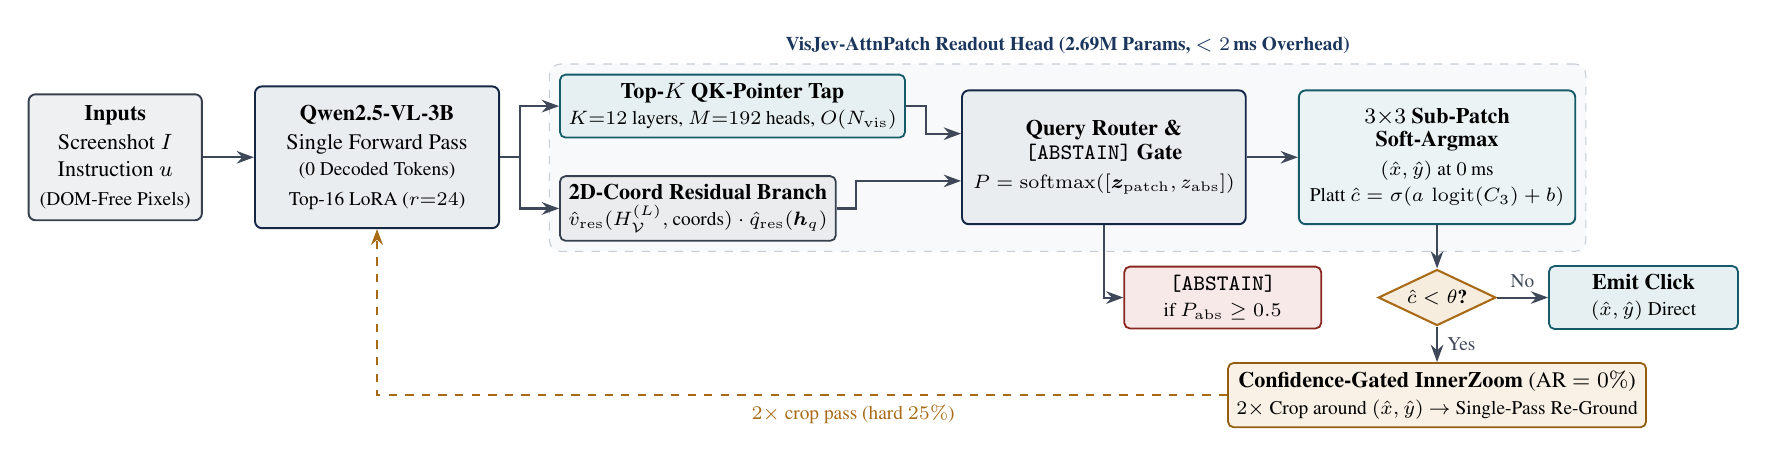
\begin{tikzpicture}[
  font=\footnotesize,
  node distance=5mm and 6mm,
  box/.style={
    draw=#1!75!black, fill=#1!9, rounded corners=2.5pt,
    line width=0.7pt, align=center, inner sep=4pt, minimum height=9mm
  },
  smallbox/.style={
    draw=#1!75!black, fill=#1!11, rounded corners=2pt,
    line width=0.65pt, align=center, inner sep=3pt, minimum height=7mm
  },
  gate/.style={
    draw=amber!85!black, fill=amber!14, diamond, aspect=2.1,
    line width=0.75pt, align=center, inner sep=1.5pt, font=\scriptsize\bfseries
  },
  arr/.style={-{Stealth[length=2.2mm,width=1.6mm]}, line width=0.75pt, color=slate!85!black},
  darr/.style={-{Stealth[length=2.0mm,width=1.5mm]}, line width=0.7pt, dashed, color=amber!85!black}
]

% 1. Input
\node[box=slate, minimum width=22mm, minimum height=16mm] (input) {
  \textbf{Inputs}\\[1pt]
  Screenshot $I$\\
  Instruction $u$\\[1pt]
  {\scriptsize (DOM-Free Pixels)}
};

% 2. VLM Backbone
\node[box=navy, right=6.5mm of input, minimum width=31mm, minimum height=18mm] (vlm) {
  \textbf{Qwen2.5-VL-3B}\\[1pt]
  Single Forward Pass\\
  {\scriptsize (0 Decoded Tokens)}\\[1pt]
  {\scriptsize Top-16 LoRA ($r{=}24$)}
};

% 3. Dual Readout Branches
\node[smallbox=teal, right=7.5mm of vlm, yshift=6.5mm, minimum width=35mm] (qk) {
  \textbf{Top-$K$ QK-Pointer Tap}\\
  {\scriptsize $K{=}12$ layers, $M{=}192$ heads, $O(N_{\mathrm{vis}})$}
};

\node[smallbox=slate, right=7.5mm of vlm, yshift=-6.5mm, minimum width=35mm] (res) {
  \textbf{2D-Coord Residual Branch}\\
  {\scriptsize $\hat{v}_{\mathrm{res}}(H^{(L)}_{\mathcal{V}},\text{coords}) \cdot \hat{q}_{\mathrm{res}}(\bm{h}_q)$}
};

% 4. Fusion + Abstention
\node[box=navy, right=7mm of qk, yshift=-6.5mm, minimum width=31mm, minimum height=17mm] (router) {
  \textbf{Query Router \&}\\[-1pt]
  \textbf{\texttt{[ABSTAIN]} Gate}\\[1pt]
  {\scriptsize $P = \softmax([\bm{z}_{\mathrm{patch}}, z_{\mathrm{abs}}])$}
};

% 5. Sub-patch + Platt
\node[box=teal, right=6.5mm of router, minimum width=28mm, minimum height=17mm] (subpatch) {
  \textbf{$3{\times}3$ Sub-Patch}\\[-1pt]
  \textbf{Soft-Argmax}\\[1pt]
  {\scriptsize $(\hat{x},\hat{y})$ at $0\,\text{ms}$}\\
  {\scriptsize Platt $\hat{c}=\sigma(a\,\logit(C_3)+b)$}
};

% 6. Decision Gate & Outputs
\node[gate, below=5.5mm of subpatch] (confgate) {$\hat{c} < \theta$?};

\node[smallbox=crimson, left=7mm of confgate, minimum width=25mm] (abstain) {
  \textbf{\texttt{[ABSTAIN]}}\\
  {\scriptsize if $P_{\mathrm{abs}} \ge 0.5$}
};

\node[smallbox=teal, right=6.5mm of confgate, minimum width=24mm] (click) {
  \textbf{Emit Click}\\
  {\scriptsize $(\hat{x},\hat{y})$ Direct}
};

\node[smallbox=amber, below=4.5mm of confgate, minimum width=46mm] (zoom) {
  \textbf{Confidence-Gated InnerZoom} (AR $=0\%$)\\
  {\scriptsize $2{\times}$ Crop around $(\hat{x},\hat{y})$ $\rightarrow$ Single-Pass Re-Ground}
};

% Arrows
\draw[arr] (input) -- (vlm);
\draw[arr] (vlm.east) -- ++(2.5mm,0) |- (qk.west);
\draw[arr] (vlm.east) -- ++(2.5mm,0) |- (res.west);
\draw[arr] (qk.east) -- ++(2.5mm,0) |- ($(router.west)+(0,3mm)$);
\draw[arr] (res.east) -- ++(2.5mm,0) |- ($(router.west)+(0,-3mm)$);
\draw[arr] (router) -- (subpatch);
\draw[arr] (subpatch) -- (confgate);
\draw[arr] (router.south) |- (abstain.west);
\draw[arr] (confgate.east) -- node[above,font=\scriptsize]{No} (click.west);
\draw[arr] (confgate.south) -- node[right,font=\scriptsize]{Yes} (zoom.north);
\draw[darr] (zoom.west) -| node[pos=0.22,below,font=\scriptsize,color=amber!85!black]{$2{\times}$ crop pass (hard $25\%$)} (vlm.south);

% Background grouping
\begin{scope}[on background layer]
  \node[draw=navy!25, fill=navy!3, rounded corners=4pt, dashed,
        fit=(qk)(res)(router)(subpatch), inner sep=3.5pt,
        label={[font=\scriptsize\bfseries\color{navy}]above:VisJev-AttnPatch Readout Head (2.69M Params, $<2$\,ms Overhead)}] {};
\end{scope}

\end{tikzpicture}%
}
\caption{Overview of the \textbf{VisJev-AttnPatch} architecture. Given raw pixels $I$ and an instruction $u$, a single forward pass of Qwen2.5-VL-3B-Instruct ($0$ decoded tokens) taps $M{=}192$ pretrained $Q/K$ attention pointer heads across the top $K{=}12$ decoder layers in $O(N_{\mathrm{vis}})$ time, fuses them with a 2D-coordinate residual branch and a learnable \texttt{[ABSTAIN]} gate, and computes continuous click coordinates $(\hat{x},\hat{y})$ via zero-cost $3{\times}3$ sub-patch soft-argmax. Only uncertain non-abstain predictions ($\hat{c} < \theta$) trigger a pure-vision $2{\times}$ \textbf{InnerZoom} pass.}
\label{fig:arch}
\end{figure*}

% =========================================================================
% SECTION 1: INTRODUCTION
% =========================================================================
\section{Introduction}
Autonomous GUI agents increasingly operate directly on raw screen pixels without relying on fragile DOM trees or OS accessibility APIs \cite{guiactor,guirlvg}. While modern VLMs such as \href{https://qwenlm.github.io/blog/qwen2.5-vl/}{Qwen2.5-VL-3B-Instruct} attain strong zero-shot grounding accuracy ($87.00\%$ on ScreenSpot-v2), standard deployment requires autoregressively generating $25\text{--}45$ text tokens for every single click. On a single NVIDIA L4 GPU, this consumes \textbf{2,151.2\,ms} per action---a severe bottleneck for real-time desktop and mobile control. Moreover, autoregressive coordinate generators are forced to output a coordinate pair even when the requested UI element does not exist on the current screen, causing destructive mis-clicks in multi-step trajectories.

Recent single-pass decision and grounding paradigms---including \href{https://github.com/microsoft/GUI-Actor}{GUI-Actor} \cite{guiactor}, \href{https://arxiv.org/html/2610.05185v1}{ReLaViS} \cite{relavis}, \href{https://aclanthology.org/2026.emnlp-main.843.pdf}{InnerZoom} \cite{innerzoom}, and System-1 decision models such as \href{https://arxiv.org/html/2610.02076v3}{LLM-as-Jev} \cite{llmasjev}---demonstrate that replacing multi-token generation with single-pass probability readout over discrete options dramatically accelerates inference. However, naive visual heads trained atop frozen VLM hidden states suffer from \emph{causal collapse} ($7.50\%$ accuracy), coarse patch-grid quantization limits small-icon precision, and existing single-pass models lack calibrated refusal.

We address these three bottlenecks with \textbf{VisJev-AttnPatch} (Figure~\ref{fig:arch}), making the following contributions:
\begin{itemize}
  \setlength{\itemsep}{2pt}\setlength{\parskip}{0pt}
  \item \textbf{$O(N_{\mathrm{vis}})$ Pretrained QK-Attention Pointer Routing:} Extracts query-to-visual attention logits directly from the VLM's top-$12$ pretrained $q_{\mathrm{proj}}/k_{\mathrm{proj}}$ layers in one FlashAttention/SDPA pass, lifting ablation accuracy from \textbf{7.00\%} to \textbf{77.33\%}.
  \item \textbf{Zero-Cost Sub-Patch Soft-Argmax \& Gaussian Soft Targets:} Eliminates patch-center quantization, adding \textbf{+6.00\%} accuracy ($n{=}300$; \textbf{+4.17\%} across all $1{,}272$ ScreenSpot-v2 samples) at \textbf{0\,ms} extra latency.
  \item \textbf{Calibrated Abstention \& Pure-Vision InnerZoom:} Achieves \textbf{0.9719--0.9778 AUROC} on mismatched instructions, \textbf{0.0776 ECE}, and \textbf{85.67\%} grounding accuracy at \textbf{5.28$\times$} mean speedup with $0\%$ autoregressive fallback.
\end{itemize}

% =========================================================================
% SECTION 2: METHOD
% =========================================================================
\section{Method: VisJev-AttnPatch Architecture}
\label{sec:method}
Given a raw screenshot $I$ and a natural-language instruction $u$, VisJev-AttnPatch executes a \textbf{single forward pass} ($0$ decoded tokens) through Qwen2.5-VL-3B-Instruct, producing $N_{\mathrm{vis}} = H_g W_g$ visual patch tokens indexed by $\mathcal{V}$ over an $H_g \times W_g$ spatial grid, alongside the final instruction token $t_{\mathrm{end}}$.

\subsection{Pretrained QK-Attention Pointer Readout}
Training a disconnected visual projection head on top of frozen final-layer hidden states fails because causal self-attention collapses spatial alignment into text-generation features. Instead, we tap the pre-attention hidden states $H^{(l)} \in \mathbb{R}^{L \times D}$ entering each of the top $K{=}12$ decoder layers ($M{=}192$ attention heads across layers $24\text{--}35$). Reusing each layer's own $\RMSNorm^{(l)}$, query projection $W_Q^{(l)}$, and GQA-expanded key projection $W_K^{(l)}$, we compute query-to-visual projections exclusively between $t_{\mathrm{end}}$ and $\mathcal{V}$:
\begin{align}
  \bm{q}^{(l)} &= W_Q^{(l)}\!\left(\RMSNorm^{(l)}\!\left(H^{(l)}_{t_{\mathrm{end}}}\right)\right), \label{eq:q_proj} \\
  K_{\mathrm{vis}}^{(l)} &= W_K^{(l)}\!\left(\RMSNorm^{(l)}\!\left(H^{(l)}_{\mathcal{V}}\right)\right). \label{eq:k_proj}
\end{align}
For each head $h$ at layer $l$ (flattened index $m \in \{1,\dots,M\}$), we compute scaled dot-product pointer logits and apply per-head $z$-score normalization across visual patches:
\begin{align}
  A^{(l)}_h &= \frac{\bm{q}^{(l)}_h \left(K_{\mathrm{vis}, h}^{(l)}\right)^{\!\top}}{\sqrt{d_h}}, \label{eq:attn_score} \\
  \tilde{A}_{m} &= \frac{A_m - \mu(A_m)}{\sigma(A_m) + \epsilon}. \label{eq:attn_norm}
\end{align}
Because Eq.~\eqref{eq:attn_score} evaluates only a single query vector against $N_{\mathrm{vis}}$ visual keys rather than materializing an $L \times L$ attention matrix, stacking $\tilde{A} \in \mathbb{R}^{M \times N_{\mathrm{vis}}}$ runs in $O(N_{\mathrm{vis}})$ time ($<2$\,ms overhead) while remaining compatible with FlashAttention/SDPA and flowing gradients directly into top-$16$ layer LoRA adapters ($r{=}24$, layers $20\text{--}35$).

\subsection{Query-Conditioned Router and Abstention Gate}
Different UI instructions (e.g., text links vs.\ small toolbar icons) rely on distinct subsets of attention heads. We construct a pooled query representation
\begin{equation}
  \bm{h}_q = \frac{1}{2}\,H^{(L)}_{t_{\mathrm{end}}} + \frac{1}{2}\,\Mean\!\left(H^{(L)}_{>\mathcal{V}}\right),
  \label{eq:hq}
\end{equation}
and predict head-routing weights $\bm{w} = \softmax(f_{\mathrm{route}}(\bm{h}_q) + \bm{b}_{\mathrm{prior}}) \in \Delta^{M-1}$. The routed pointer map is fused with a lightweight 2D-coordinate residual branch to obtain per-patch logits $\bm{z}_{\mathrm{patch}} \in \mathbb{R}^{N_{\mathrm{vis}}}$:
\begin{align}
  \bm{z}_{\mathrm{patch}} &= \tau \sum_{m=1}^{M} w_m \tilde{A}_m \nonumber \\
  &\quad + \gamma \left(\hat{v}_{\mathrm{res}}\!\left(H^{(L)}_{\mathcal{V}},\, \mathrm{coords}\right) \cdot \hat{q}_{\mathrm{res}}(\bm{h}_q)\right),
  \label{eq:zpatch}
\end{align}
where $\tau$ and $\gamma$ are learnable scaling parameters.

To enable calibrated refusal when a target element is absent from the screen, an auxiliary MLP maps the concatenated global context and spatial distribution statistics to a scalar abstention logit:
\begin{equation}
  z_{\mathrm{abstain}} = \MLP\!\left(\left[\bm{h}_q;\; \bm{v}_{\mathrm{att}};\; \max(\bm{z}_{\mathrm{patch}});\; \mathcal{H}(p)\right]\right),
  \label{eq:abstain}
\end{equation}
where $\bm{v}_{\mathrm{att}}$ is the attention-pooled visual feature and $\mathcal{H}(p)$ is the Shannon entropy of the patch distribution. Joint normalization yields $P = \softmax([\bm{z}_{\mathrm{patch}},\, z_{\mathrm{abstain}}])$.

\subsection{Gaussian Soft Targets \& Sub-Patch Refinement}
Discrete patch classification penalizes predictions that fall on adjacent patches overlapping the target bounding box. During training, positive examples use a 2D Gaussian-smoothed spatial target:
\begin{equation}
  \bm{y} = 0.75\,\bm{y}_{\mathrm{box}} + 0.25\,\bm{y}_{\mathcal{N}}(\sigma{=}1.0),
  \label{eq:softtarget}
\end{equation}
while $20\%$ hard-negative instruction--screenshot pairs supervise $z_{\mathrm{abstain}}$.

At inference time, rather than clicking the center of the discrete argmax patch $(r^*, c^*)$, we extract the $3{\times}3$ local neighborhood $\mathcal{N}_3$ around $(r^*, c^*)$, compute its total probability mass $C_3 = \sum_{(r,c)\in\mathcal{N}_3} P_{r,c}$, and obtain continuous sub-patch coordinates at \textbf{0\,ms} extra latency:
\begin{equation}
  (\hat{x}, \hat{y}) = \frac{1}{C_3} \sum_{(r,c)\in\mathcal{N}_3} P_{r,c} \left(\frac{c + 0.5}{W_g},\; \frac{r + 0.5}{H_g}\right).
  \label{eq:subpatch}
\end{equation}

% =========================================================================
% TABLE 1: MAIN COMPARISON (Full Width, Page 3 Top — zero overflow!)
% =========================================================================
\begin{table*}[t]
\centering
\caption{Controlled ($n{=}300$) and full-benchmark ($n{=}1{,}272$) zero-shot evaluation on ScreenSpot-v2 (NVIDIA L4 GPU, $768$-token visual budget unless noted). Best single-pass/pure-vision metrics in each section are highlighted in \textbf{bold}.}
\label{tab:main}
\footnotesize
\setlength{\tabcolsep}{3.6pt}
\begin{tabular}{@{}lcccccc@{}}
\toprule
\textbf{Method} & \textbf{Overall Acc $\uparrow$} & \textbf{Text / Icon} & \textbf{Med.\ Lat.\ (ms) $\downarrow$} & \textbf{Speedup $\uparrow$} & \textbf{ECE $\downarrow$} & \textbf{Abstain AUROC $\uparrow$} \\
\midrule
\multicolumn{7}{@{}l}{\textit{\color{slate}Controlled Zero-Shot Evaluation ($n{=}300$ unless noted)}} \\
Baseline A: Official Qwen2.5-VL-3B AR ($n{=}100$) & 87.00\% & 94.64\% / 77.27\% & 2,151.2 & 1.00$\times$ & --- & --- \\
Phase 1: Frozen Backbone + 3.98M Head ($n{=}200$) & 7.50\% & 8.40\% / 6.17\% & 318.1 & 6.76$\times$ & 0.3366 & 0.5287 \\
Phase 4: VisJev-AttnPatch v4 (512 Fast) & 72.33\% & 80.61\% / 62.22\% & \textbf{233.4} & \textbf{9.22$\times$} & 0.1366 & 0.9674 \\
Phase 4: VisJev-AttnPatch v4 (768 Res.) & 77.00\% & 87.27\% / 64.44\% & 337.6 & 6.37$\times$ & 0.0880 & \textbf{0.9778} \\
Phase 6: VisJev-AttnPatch v6 (Gaussian, Discrete) & 77.33\% & 86.06\% / 66.67\% & 332.8 & 6.46$\times$ & \textbf{0.0776} & 0.9719 \\
\rowcolor{rowhl}
\textbf{Phase 7: VisJev-v6 + 0\,ms Sub-Patch} & 83.33\% & --- & 327.7 & 6.56$\times$ & \textbf{0.0776} & 0.9719 \\
\rowcolor{rowhl}
\textbf{Phase 7: VisJev-v6 + InnerZoom ($\theta{=}0.82$, AR\,=\,0\%)} & \textbf{85.67\%} & --- & 335.9 & 5.28$\times$\textsuperscript{$\dagger$} & \textbf{0.0776} & 0.9719 \\
\midrule
\multicolumn{7}{@{}l}{\textit{\color{slate}Full ScreenSpot-v2 Zero-Shot Benchmark ($n{=}1{,}272$, 718 Text / 554 Icon)}} \\
VisJev-v6 Discrete Single-Pass & 77.75\% & --- & 331.6 & 6.49$\times$ & --- & --- \\
\rowcolor{rowhl}
\textbf{VisJev-v6 + 0\,ms Sub-Patch Single-Pass} & 81.92\% & 89.26\% / 70.64\% & \textbf{331.6} & \textbf{6.49$\times$} & --- & --- \\
\rowcolor{rowhl}
\textbf{VisJev-v6 + InnerZoom ($\theta{=}0.85$, 46.5\% esc.)} & \textbf{83.02\%} & \textbf{90.02\% / 72.18\%} & 356.5 & 6.03$\times$ & --- & --- \\
\bottomrule
\end{tabular}
\begin{flushleft}
\vspace{-4pt}
{\scriptsize \textsuperscript{$\dagger$}Mean speedup ($2{,}151.2 / 407.4\,\text{ms} = 5.28\times$); median speedup is $6.40\times$ ($335.9\,\text{ms}$).}
\end{flushleft}
\end{table*}

\subsection{Platt Calibration \& Pure-Vision InnerZoom}
We calibrate raw neighborhood mass $C_3$ via post-hoc Platt scaling fitted on validation logits ($a{=}0.352$, $b{=}1.991$):
\begin{equation}
  \hat{c} = \sigma\!\left(a\,\logit(C_3) + b\right).
  \label{eq:platt}
\end{equation}
As summarized in Algorithm~1, when $P_{\mathrm{abstain}} \ge 0.5$, the agent abstains. Otherwise, high-confidence predictions ($\hat{c} \ge \theta$) emit $(\hat{x},\hat{y})$ immediately in a single pass, whereas uncertain predictions ($\hat{c} < \theta$) escalate to \textbf{Confidence-Gated InnerZoom}: cropping a $2{\times}$ region centered at $(\hat{x},\hat{y})$ and re-running the exact same single-pass pointer readout without invoking autoregressive decoding.

% --- Ruled Academic Algorithm Block (clean raggedright, no duplicate Figure caption) ---
\begin{figure}[t]
\centering
\footnotesize
\begin{tabular}{@{} >{\raggedright\arraybackslash}p{\dimexpr\linewidth\relax} @{}}
\toprule
\textbf{Algorithm 1:} VisJev-AttnPatch Single-Pass \& InnerZoom Inference \\
\midrule
\textbf{Input:} Screenshot $I$, instruction $u$, threshold $\theta$, Platt $(a,b)$ \\
\textbf{Output:} Continuous click $(\hat{x},\hat{y})$ or \texttt{[ABSTAIN]} \\[2pt]
\makebox[1.4em][r]{1:}\hspace{0.4em}Run single VLM forward pass on $(I,u)$ ($0$ decoded tokens). \\
\makebox[1.4em][r]{2:}\hspace{0.4em}Tap top-$K$ QK pointer maps $\tilde{A}$ via Eqs.~\eqref{eq:q_proj}--\eqref{eq:attn_norm}. \\
\makebox[1.4em][r]{3:}\hspace{0.4em}Compute $\bm{z}_{\mathrm{patch}}, z_{\mathrm{abstain}}$ via Eqs.~\eqref{eq:hq}--\eqref{eq:abstain}. \\
\makebox[1.4em][r]{4:}\hspace{0.4em}$P \gets \softmax([\bm{z}_{\mathrm{patch}},\, z_{\mathrm{abstain}}])$. \\
\makebox[1.4em][r]{5:}\hspace{0.4em}\textbf{if} $P_{\mathrm{abstain}} \ge 0.5$ \textbf{then return} \texttt{[ABSTAIN]}. \\
\makebox[1.4em][r]{6:}\hspace{0.4em}Compute $(\hat{x},\hat{y})$ and mass $C_3$ over $\mathcal{N}_3$ via Eq.~\eqref{eq:subpatch}. \\
\makebox[1.4em][r]{7:}\hspace{0.4em}$\hat{c} \gets \sigma(a\,\logit(C_3) + b)$ \hfill {\color{slate}\textit{// Platt calibration}} \\
\makebox[1.4em][r]{8:}\hspace{0.4em}\textbf{if} $\hat{c} < \theta$ \textbf{then} \hfill {\color{slate}\textit{// Pure-vision InnerZoom}} \\
\makebox[1.4em][r]{9:}\hspace{1.4em}$I_{\mathrm{crop}} \gets \mathrm{Crop2x}(I, \hat{x}, \hat{y})$. \\
\makebox[1.4em][r]{10:}\hspace{1.4em}$(\hat{x}_{\mathrm{loc}}, \hat{y}_{\mathrm{loc}}) \gets \mathrm{SinglePassSubPatch}(I_{\mathrm{crop}}, u)$. \\
\makebox[1.4em][r]{11:}\hspace{1.4em}Map $(\hat{x}_{\mathrm{loc}}, \hat{y}_{\mathrm{loc}})$ back to global $(\hat{x},\hat{y})$. \\
\makebox[1.4em][r]{12:}\hspace{0.4em}\textbf{return} $(\hat{x}, \hat{y})$. \\
\bottomrule
\end{tabular}
\end{figure}

% =========================================================================
% FIGURE 2: PARETO FRONTIER + ABLATION (Full Width, Page 3/4 Top — zero label overlap!)
% =========================================================================
\begin{figure*}[t]
\centering
\begin{subfigure}[t]{0.52\textwidth}
\centering
\resizebox{\linewidth}{!}{%
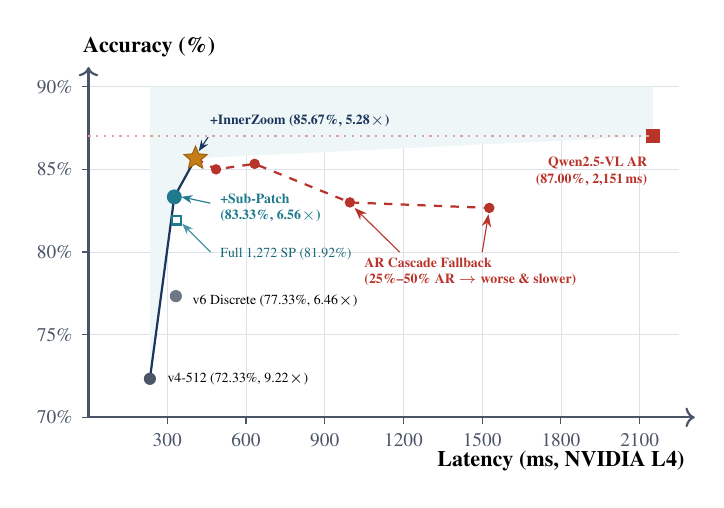
\begin{tikzpicture}[font=\scriptsize]
  % Plot frame: x in [0, 7.6] maps latency [0, 2300] ms; y in [0, 4.4] maps acc [70, 90]%
  % Scale: x_coord = lat / 300.0; y_coord = (acc - 70.0) * 0.21
  \draw[gridgray, very thin] (0,0) grid[xstep=1.0, ystep=1.05] (7.5,4.2);
  \draw[->, thick, slate] (0,0) -- (7.7,0) node[below left, yshift=-3mm, font=\footnotesize\bfseries, color=black]{Latency (ms, NVIDIA L4)};
  \draw[->, thick, slate] (0,0) -- (0,4.45) node[above right, xshift=-2mm, font=\footnotesize\bfseries, color=black]{Accuracy (\%)};

  % X ticks: 300..2100
  \foreach \lat/\xl in {300/1.0, 600/2.0, 900/3.0, 1200/4.0, 1500/5.0, 1800/6.0, 2100/7.0}{
    \draw[slate] (\xl, 0) -- (\xl, -0.08) node[below]{\lat};
  }
  % Y ticks: 70..90
  \foreach \acc/\yl in {70/0.0, 75/1.05, 80/2.10, 85/3.15, 90/4.20}{
    \draw[slate] (0, \yl) -- (-0.08, \yl) node[left]{\acc\%};
  }

  % Shaded Pareto region
  \fill[teal!7] (0.78, 0.49) -- (1.09, 2.80) -- (1.36, 3.29) -- (7.17, 3.57) -- (7.17, 4.2) -- (0.78, 4.2) -- cycle;

  % Cascade Curve (AR fallback degradation)
  \draw[crimson, thick, dashed] (1.36,3.29) -- (1.62,3.15) -- (2.11,3.22) -- (3.32,2.73) -- (5.09,2.66);
  \foreach \x/\y in {1.62/3.15, 2.11/3.22, 3.32/2.73, 5.09/2.66}{
    \fill[crimson] (\x,\y) circle (1.9pt);
  }
  \node[crimson, align=left, font=\tiny\bfseries] at (4.85, 1.85) {AR Cascade Fallback\\(25\%--50\% AR $\rightarrow$ worse \& slower)};
  \draw[-{Stealth[length=1.6mm]}, crimson, thin] (3.95,2.10) -- (3.38,2.66);
  \draw[-{Stealth[length=1.6mm]}, crimson, thin] (5.00,2.10) -- (5.08,2.58);

  % Pareto Curve (Pure-vision)
  \draw[navy, thick] (0.78,0.49) -- (1.09,2.80) -- (1.36,3.29);

  % Points & clean non-overlapping labels:
  % 1. v4-512: (233.4, 72.33) -> (0.78, 0.49)
  \fill[slate] (0.78,0.49) circle (2.2pt);
  \node[right, font=\tiny] at (0.88, 0.49) {v4-512 (72.33\%, 9.22$\times$)};

  % 2. v6 Discrete: (332.8, 77.33) -> (1.11, 1.54)
  \fill[slate!80] (1.11,1.54) circle (2.2pt);
  \node[right, font=\tiny] at (1.20, 1.48) {v6 Discrete (77.33\%, 6.46$\times$)};

  % 3. Full 1,272 SP: (331.6, 81.92) -> (1.11, 2.50)
  \draw[teal, fill=white, thick] (1.06, 2.45) rectangle ++(0.11, 0.11);
  \node[right, font=\tiny, color=teal!85!black] at (1.55, 2.08) {Full 1,272 SP (81.92\%)};
  \draw[-{Stealth[length=1.4mm]}, teal!80, thin] (1.55,2.10) -- (1.19,2.46);

  % 4. +Sub-Patch n=300: (327.7, 83.33) -> (1.09, 2.80)
  \fill[teal] (1.09,2.80) circle (2.7pt);
  \node[right, align=left, font=\tiny\bfseries, color=teal] at (1.55, 2.66) {+Sub-Patch\\(83.33\%, 6.56$\times$)};
  \draw[-{Stealth[length=1.4mm]}, teal, thin] (1.55,2.72) -- (1.18,2.80);

  % 5. +InnerZoom n=300: (407.4 mean, 85.67) -> (1.36, 3.29)
  \node[star, star points=5, star point ratio=2.2, fill=amber, draw=amber!80!black, inner sep=1.4pt] (iz) at (1.36,3.29) {};
  \node[above right, font=\tiny\bfseries, color=navy] at (1.42, 3.56) {+InnerZoom (85.67\%, 5.28$\times$)};
  \draw[-{Stealth[length=1.4mm]}, navy, thin] (1.52,3.56) -- (1.40,3.38);

  % 6. Autoregressive Baseline: (2151.2, 87.00) -> (7.17, 3.57)
  \fill[crimson] (7.17,3.57) ++(-2.5pt,-2.5pt) rectangle ++(5pt,5pt);
  \node[below left, font=\tiny\bfseries, color=crimson, align=right] at (7.22, 3.43) {Qwen2.5-VL AR\\(87.00\%, 2,151\,ms)};

  \draw[crimson!45, dotted, thick] (0,3.57) -- (7.17,3.57);
\end{tikzpicture}%
}
\caption{Accuracy--Latency Pareto frontier and 3-tier AR cascade.}
\label{fig:pareto}
\end{subfigure}%
\hfill
\begin{subfigure}[t]{0.39\textwidth}
\centering
\resizebox{\linewidth}{!}{%
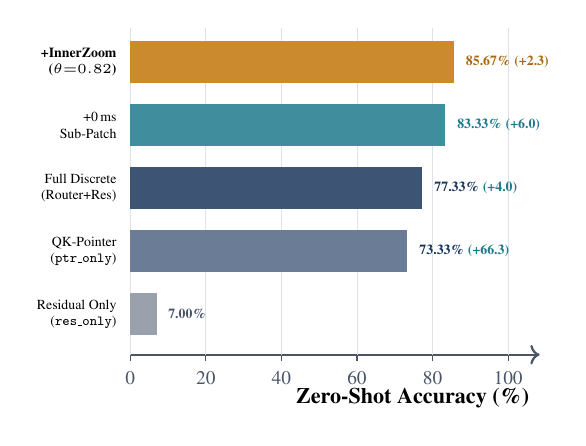
\begin{tikzpicture}[font=\scriptsize]
  % Horizontal bar chart: x in [0, 5.2] maps [0, 100]% (x = acc * 0.048)
  \draw[->, thick, slate] (0,0) -- (5.20,0) node[below left, yshift=-3mm, font=\footnotesize\bfseries, color=black]{Zero-Shot Accuracy (\%)};
  \foreach \v/\x in {0/0, 20/0.96, 40/1.92, 60/2.88, 80/3.84, 100/4.80}{
    \draw[gridgray, very thin] (\x, 0) -- (\x, 4.15);
    \draw[slate] (\x, 0) -- (\x, -0.08) node[below]{\v};
  }

  % Bars (bottom to top)
  \fill[slate!55] (0, 0.25) rectangle (0.336, 0.78);
  \node[left, align=right, font=\tiny] at (-0.05, 0.515) {Residual Only\\(\texttt{res\_only})};
  \node[right, font=\tiny\bfseries, color=slate] at (0.36, 0.515) {7.00\%};

  \fill[navy!65] (0, 1.05) rectangle (3.520, 1.58);
  \node[left, align=right, font=\tiny] at (-0.05, 1.315) {QK-Pointer\\(\texttt{ptr\_only})};
  \node[right, font=\tiny\bfseries, color=navy] at (3.55, 1.315) {73.33\% \textcolor{teal}{(+66.3)}};

  \fill[navy!85] (0, 1.85) rectangle (3.712, 2.38);
  \node[left, align=right, font=\tiny] at (-0.05, 2.115) {Full Discrete\\(Router+Res)};
  \node[right, font=\tiny\bfseries, color=navy] at (3.74, 2.115) {77.33\% \textcolor{teal}{(+4.0)}};

  \fill[teal!85] (0, 2.65) rectangle (4.000, 3.18);
  \node[left, align=right, font=\tiny] at (-0.05, 2.915) {+0\,ms\\Sub-Patch};
  \node[right, font=\tiny\bfseries, color=teal] at (4.03, 2.915) {83.33\% \textcolor{teal}{(+6.0)}};

  \fill[amber!90] (0, 3.45) rectangle (4.112, 3.98);
  \node[left, align=right, font=\tiny\bfseries] at (-0.05, 3.715) {+InnerZoom\\($\theta{=}0.82$)};
  \node[right, font=\tiny\bfseries, color=amber!85!black] at (4.14, 3.715) {85.67\% \textcolor{amber!85!black}{(+2.3)}};
\end{tikzpicture}%
}
\caption{Progressive component ablation ($n{=}300$).}
\label{fig:ablation}
\end{subfigure}
\caption{\textbf{Efficiency--accuracy trade-off and ablation on ScreenSpot-v2 ($n{=}300$, NVIDIA L4).} (a) VisJev-AttnPatch with $0$\,ms sub-patch refinement and pure-vision InnerZoom establishes a sharp Pareto frontier, whereas cascading to autoregressive Qwen2.5-VL-3B on uncertain samples increases latency up to $1{,}526$\,ms while degrading accuracy to $82.67\%$. (b) Tapping pretrained QK pointer heads delivers the decisive $+66.33\%$ leap over a standalone residual head, followed by steady gains from fusion, sub-patch soft-argmax, and InnerZoom.}
\label{fig:main_plots}
\end{figure*}

% =========================================================================
% SECTION 3: EXPERIMENTS
% =========================================================================
\section{Experimental Setup \& Results}
\label{sec:exp}

\subsection{Training Data \& Evaluation Protocol}
We train VisJev-AttnPatch on only \textbf{1,200 unique filtered web samples} from \href{https://huggingface.co/datasets/Voxel51/WaveUI-25k}{WaveUI-25k}, using rich semantic \texttt{purpose}/\texttt{description} fields rather than noisy generic \texttt{instruction} accessibility tags. Training runs in \textbf{29\,minutes} on a single NVIDIA L4 GPU, updating only $0.13\%$ LoRA parameters ($r{=}24$, layers $20\text{--}35$) plus the $2.69\text{M}$-parameter pointer/abstention head ($30.5\,\text{MB}$ checkpoint). We evaluate strictly \textbf{zero-shot} on \href{https://huggingface.co/datasets/lmms-lab/ScreenSpot-v2}{ScreenSpot-v2} ($n{=}1{,}272$ full benchmark across $8$ desktop, mobile, and web platforms; $n{=}300$ controlled suite with calibration and abstention stress tests) and \href{https://huggingface.co/datasets/HongxinLi/ScreenSpot-Pro}{ScreenSpot-Pro} ($n{=}200$ 4K professional software).

% =========================================================================
% FIGURE 3: FULL 1,272 PLATFORM BREAKDOWN (Full Width, placed cleanly before Conclusion)
% =========================================================================
\begin{figure*}[t]
\centering
\resizebox{0.88\textwidth}{!}{%
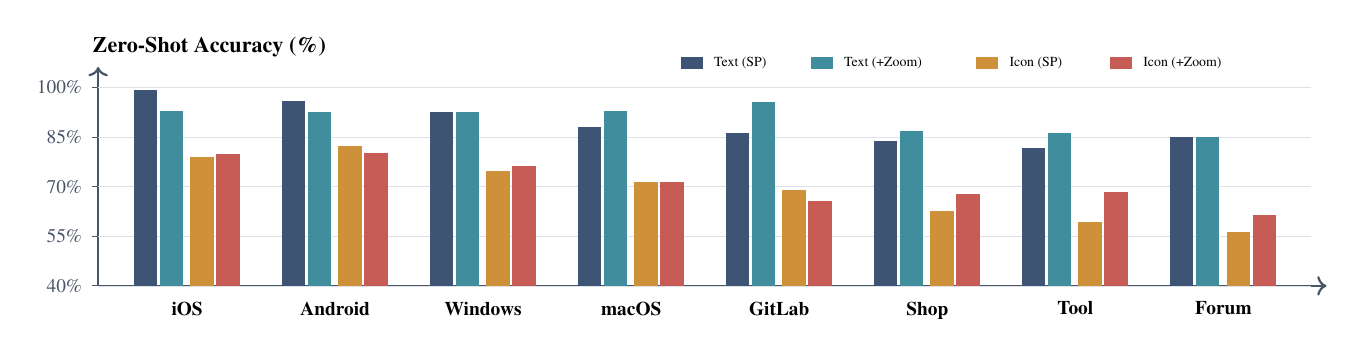
\begin{tikzpicture}[font=\scriptsize]
  % 8 platform groups across x in [0, 15.2], y in [0, 2.75] maps [40, 100]% -> y = (val - 40) * 0.042
  \draw[->, thick, slate] (0,0) -- (15.6,0);
  \draw[->, thick, slate] (0,0) -- (0,2.78) node[above right, xshift=-2mm, font=\footnotesize\bfseries, color=black]{Zero-Shot Accuracy (\%)};

  \foreach \v/\y in {40/0.0, 55/0.63, 70/1.26, 85/1.89, 100/2.52}{
    \draw[gridgray, very thin] (0, \y) -- (15.4, \y);
    \draw[slate] (0, \y) -- (-0.08, \y) node[left]{\v\%};
  }

  % Legend at top right
  \begin{scope}[shift={(7.4, 2.75)}]
    \fill[navy!85] (0,0) rectangle (0.28,0.16); \node[right, font=\tiny] at (0.30,0.08) {Text (SP)};
    \fill[teal!85] (1.65,0) rectangle (1.93,0.16); \node[right, font=\tiny] at (1.95,0.08) {Text (+Zoom)};
    \fill[amber!85] (3.75,0) rectangle (4.03,0.16); \node[right, font=\tiny] at (4.05,0.08) {Icon (SP)};
    \fill[crimson!80] (5.45,0) rectangle (5.73,0.16); \node[right, font=\tiny] at (5.75,0.08) {Icon (+Zoom)};
  \end{scope}

  % Platforms: idx, name, t_sp, t_zm, i_sp, i_zm
  \foreach \idx/\name/\tsp/\tzm/\isp/\izm in {
    0/iOS/99.28/92.75/79.00/80.00,
    1/Android/95.83/92.50/82.42/80.22,
    2/Windows/92.71/92.71/74.60/76.19,
    3/macOS/88.10/92.86/71.43/71.43,
    4/GitLab/86.36/95.45/68.97/65.52,
    5/Shop/83.85/86.92/62.61/67.83,
    6/Tool/81.82/86.36/59.26/68.52,
    7/Forum/85.00/85.00/56.41/61.54
  }{
    \pgfmathsetmacro{\bx}{0.45 + \idx * 1.88}
    \pgfmathsetmacro{\htsp}{(\tsp - 40) * 0.042}
    \pgfmathsetmacro{\htzm}{(\tzm - 40) * 0.042}
    \pgfmathsetmacro{\hisp}{(\isp - 40) * 0.042}
    \pgfmathsetmacro{\hizm}{(\izm - 40) * 0.042}
    \fill[navy!85] (\bx, 0) rectangle (\bx+0.30, \htsp);
    \fill[teal!85] (\bx+0.33, 0) rectangle (\bx+0.63, \htzm);
    \fill[amber!85] (\bx+0.72, 0) rectangle (\bx+1.02, \hisp);
    \fill[crimson!80] (\bx+1.05, 0) rectangle (\bx+1.35, \hizm);
    \node[below, font=\scriptsize\bfseries] at (\bx+0.68, -0.08) {\name};
  }
\end{tikzpicture}%
}
\caption{Full ScreenSpot-v2 ($n{=}1{,}272$) zero-shot accuracy breakdown across all eight mobile, desktop, and web platforms comparing single-pass sub-patch grounding (SP) vs.\ Confidence-Gated InnerZoom ($\theta{=}0.85$). Pure-vision zooming yields the largest icon gains on dense web interfaces (\textbf{Tool}: $+9.26\%$, \textbf{Shop}: $+5.22\%$, \textbf{Forum}: $+5.13\%$).}
\label{fig:platforms}
\end{figure*}

\subsection{Main Grounding, Calibration \& Cascade Results}
Table~\ref{tab:main} and Figure~\ref{fig:pareto} summarize the primary results. On the controlled suite ($n{=}300$), a disconnected visual head over frozen hidden states collapses to $7.50\%$ accuracy. Introducing pretrained QK-pointer routing raises discrete single-pass accuracy to $77.33\%$ ($6.46\times$ speedup) with \textbf{0.0776 ECE} and \textbf{0.9719 abstention AUROC}. Adding zero-cost $3{\times}3$ sub-patch soft-argmax boosts accuracy by $+6.00\%$ to \textbf{83.33\%} at \textbf{327.7\,ms} median latency (\textbf{6.56$\times$ speedup}). Across all $1{,}272$ ScreenSpot-v2 samples, single-pass sub-patch grounding achieves \textbf{81.92\%} at \textbf{331.6\,ms} (\textbf{6.49$\times$ speedup}), and Confidence-Gated InnerZoom ($\theta{=}0.85$) lifts accuracy to \textbf{83.02\%} (\textbf{6.03$\times$ speedup}).

\takeawaybox{Key Finding (Pure-Vision InnerZoom vs.\ AR Cascade)}{On the hardest $25\%$ of clicks, escalating to a single-pass $2{\times}$ pure-vision InnerZoom (\textbf{85.67\%}, $407.4\,\text{ms}$ mean, $5.28\times$ speedup) \textbf{strictly outperforms} falling back to autoregressive Qwen2.5-VL-3B ($83.00\%$ at $25\%$ AR / $82.67\%$ at $50\%$ AR, $997\text{--}1{,}526\,\text{ms}$).}

Table~\ref{tab:cascade} details the 3-tier cascade sweep on $n{=}300$. Because the hardest $25\%$ of clicks consist largely of tiny, visually ambiguous icons where full-screen autoregressive decoding also loses spatial fidelity, zooming in visually at $2{\times}$ resolution solves the bottleneck far more accurately and $2.4\text{--}3.7\times$ faster than autoregressive fallback.

\begin{table}[t]
\centering
\caption{Three-tier cascade sweep ($n{=}300$, ScreenSpot-v2). Pure-vision InnerZoom ($\theta_{\mathrm{AR}}{=}0$) dominates AR fallback in both accuracy and latency.}
\label{tab:cascade}
\footnotesize
\setlength{\tabcolsep}{2.4pt}
\begin{tabular}{@{}cccccc@{}}
\toprule
$(\theta_{\mathrm{zoom}}, \theta_{\mathrm{AR}})$ & \textbf{S1/Zm/AR (\%)} & \textbf{Acc} & \textbf{Med.} & \textbf{Mean} & \textbf{Spd.} \\
\midrule
\rowcolor{rowhl}
\textbf{(0.82, 0.00)} & 75.0 / 25.0 / \textbf{0.0} & \textbf{85.67\%} & \textbf{335.9} & \textbf{407.4} & \textbf{5.28$\times$} \\
(0.85, 0.00) & 50.0 / 50.0 / 0.0 & 85.00\% & 405.6 & 486.4 & 4.42$\times$ \\
(0.85, 0.78) & 50.0 / 42.3 / 7.7 & 85.33\% & 405.6 & 631.5 & 3.41$\times$ \\
(0.86, 0.82) & 40.3 / 34.7 / 25.0 & 83.00\% & 647.9 & 997.0 & 2.16$\times$ \\
(0.88, 0.85) & 22.7 / 27.3 / 50.0 & 82.67\% & 1,500.3 & 1,526.2 & 1.41$\times$ \\
\bottomrule
\end{tabular}
\begin{flushleft}
\vspace{-4pt}
{\scriptsize Latencies (Med., Mean) in milliseconds on NVIDIA L4; speedup vs.\ 2,151.2\,ms AR.}
\end{flushleft}
\end{table}

\subsection{Component Ablation \& Platform Breakdown}
Figure~\ref{fig:ablation} isolates each architectural component on ScreenSpot-v2 ($n{=}300$). Removing the QK-pointer router leaves only the residual head (\texttt{res\_only}, $7.00\%$). Enabling pretrained QK-pointer routing alone (\texttt{ptr\_only}) jumps to $73.33\%$ ($+66.33\%$), confirming that pretrained VLM attention already encodes strong zero-shot spatial localization. Combining both branches reaches $77.33\%$ ($+4.00\%$), zero-cost $3{\times}3$ sub-patch soft-argmax adds $+6.00\%$ ($83.33\%$), and pure-vision InnerZoom ($\theta{=}0.82$) adds a further $+2.34\%$ to $85.67\%$.

Figure~\ref{fig:platforms} and Table~\ref{tab:full1272} report the complete $n{=}1{,}272$ platform breakdown. Single-pass sub-patch grounding already excels on mobile text (\textbf{99.28\%} on iOS, \textbf{95.83\%} on Android), while Confidence-Gated InnerZoom delivers substantial gains on dense web and desktop interfaces---lifting GitLab text by $+9.09\%$ ($86.36\% \rightarrow 95.45\%$) and Tool icons by $+9.26\%$ ($59.26\% \rightarrow 68.52\%$).

\begin{table}[t]
\centering
\caption{Full ScreenSpot-v2 ($n{=}1{,}272$) per-platform accuracy: Sub-Patch Single-Pass (SP) vs.\ +InnerZoom ($\theta{=}0.85$).}
\label{tab:full1272}
\footnotesize
\setlength{\tabcolsep}{3.5pt}
\begin{tabular}{@{}lrrrrr@{}}
\toprule
& \multicolumn{2}{c}{\textbf{Text (\%)}} & \multicolumn{2}{c}{\textbf{Icon (\%)}} & \textbf{Count} \\
\cmidrule(lr){2-3} \cmidrule(lr){4-5}
\textbf{Platform} & \textbf{SP} & \textbf{+Zoom} & \textbf{SP} & \textbf{+Zoom} & \textbf{(T / I)} \\
\midrule
iOS & \textbf{99.28} & 92.75 & 79.00 & \textbf{80.00} & 138 / 100 \\
Android & \textbf{95.83} & 92.50 & \textbf{82.42} & 80.22 & 120 / 91 \\
Windows & \textbf{92.71} & \textbf{92.71} & 74.60 & \textbf{76.19} & 96 / 63 \\
macOS & 88.10 & \textbf{92.86} & \textbf{71.43} & \textbf{71.43} & 84 / 63 \\
GitLab & 86.36 & \textbf{95.45} & \textbf{68.97} & 65.52 & 44 / 29 \\
Shop & 83.85 & \textbf{86.92} & 62.61 & \textbf{67.83} & 130 / 115 \\
Tool & 81.82 & \textbf{86.36} & 59.26 & \textbf{68.52} & 66 / 54 \\
Forum & \textbf{85.00} & \textbf{85.00} & 56.41 & \textbf{61.54} & 40 / 39 \\
\midrule
\rowcolor{rowhl}
\textbf{All (1,272)} & 89.26 & \textbf{90.02} & 70.64 & \textbf{72.18} & \textbf{718 / 554} \\
\bottomrule
\end{tabular}
\end{table}

% =========================================================================
% SECTION 4: CONCLUSION & LIMITATIONS
% =========================================================================
\section{Conclusion \& Limitations}
\label{sec:conclusion}
VisJev-AttnPatch demonstrates that DOM-free GUI grounding does not require slow autoregressive token decoding. With only $1{,}200$ filtered training examples and a $30.5\,\text{MB}$ adapter checkpoint, our single-pass QK-pointer architecture achieves \textbf{81.92--85.67\%} zero-shot accuracy on ScreenSpot-v2 at \textbf{5.3--6.5$\times$ lower latency}, \textbf{0.0776 ECE}, and \textbf{0.972 abstention AUROC}.

\paragraph{Limitations.}
On ultra-high-resolution 4K professional software benchmarks (\href{https://huggingface.co/datasets/HongxinLi/ScreenSpot-Pro}{ScreenSpot-Pro}, $n{=}200$), compressing full screenshots into a $768$-token visual budget remains a resolution bottleneck ($2.0\% \rightarrow 4.0\%$ with $2{\times}$ InnerZoom). Extending VisJev-AttnPatch with hierarchical multi-scale tiled attention routing is a promising direction for future work.

% =========================================================================
% REFERENCES
% =========================================================================
\begin{thebibliography}{9}
\footnotesize
\setlength{\itemsep}{1.2pt}

\bibitem{guiactor}
Q.~Wu et~al., ``GUI-Actor: Coordinate-Free Visual Grounding for GUI Agents,'' in \emph{Advances in Neural Information Processing Systems (NeurIPS)}, 2025. \url{https://github.com/microsoft/GUI-Actor}

\bibitem{relavis}
ReLaViS Authors, ``Recurrent Latent Visual Search for GUI Grounding,'' \emph{arXiv preprint arXiv:2610.05185}, 2026. \url{https://arxiv.org/html/2610.05185v1}

\bibitem{innerzoom}
InnerZoom Authors, ``InnerZoom: Intermediate Target Evidence Refinement for GUI Grounding,'' in \emph{Proceedings of EMNLP}, 2026. \url{https://aclanthology.org/2026.emnlp-main.843.pdf}

\bibitem{guirlvg}
GuirlVG Authors, ``GuirlVG: Incentivize GUI Visual Grounding via Empirical Exploration,'' \emph{arXiv preprint arXiv:2508.04389}, 2025. \url{https://arxiv.org/pdf/2508.04389}

\bibitem{llmasjev}
LLM-as-Jev Authors, ``Single-Pass Calibrated Decision Readout for Foundation Models,'' \emph{arXiv preprint arXiv:2610.02076}, 2026. \url{https://arxiv.org/html/2610.02076v3}

\end{thebibliography}

\end{document}
